\documentclass[border=15pt, tikz]{standalone}
\usepackage{tikz}
\usetikzlibrary{calc, positioning, shadows}

% Definición de la paleta de colores
\definecolor{cPurple}{HTML}{8E44AD}
\definecolor{cOrange}{HTML}{E67E22}
\definecolor{cCyan}{HTML}{5DBCD2}

\begin{document}
\pagecolor{white}
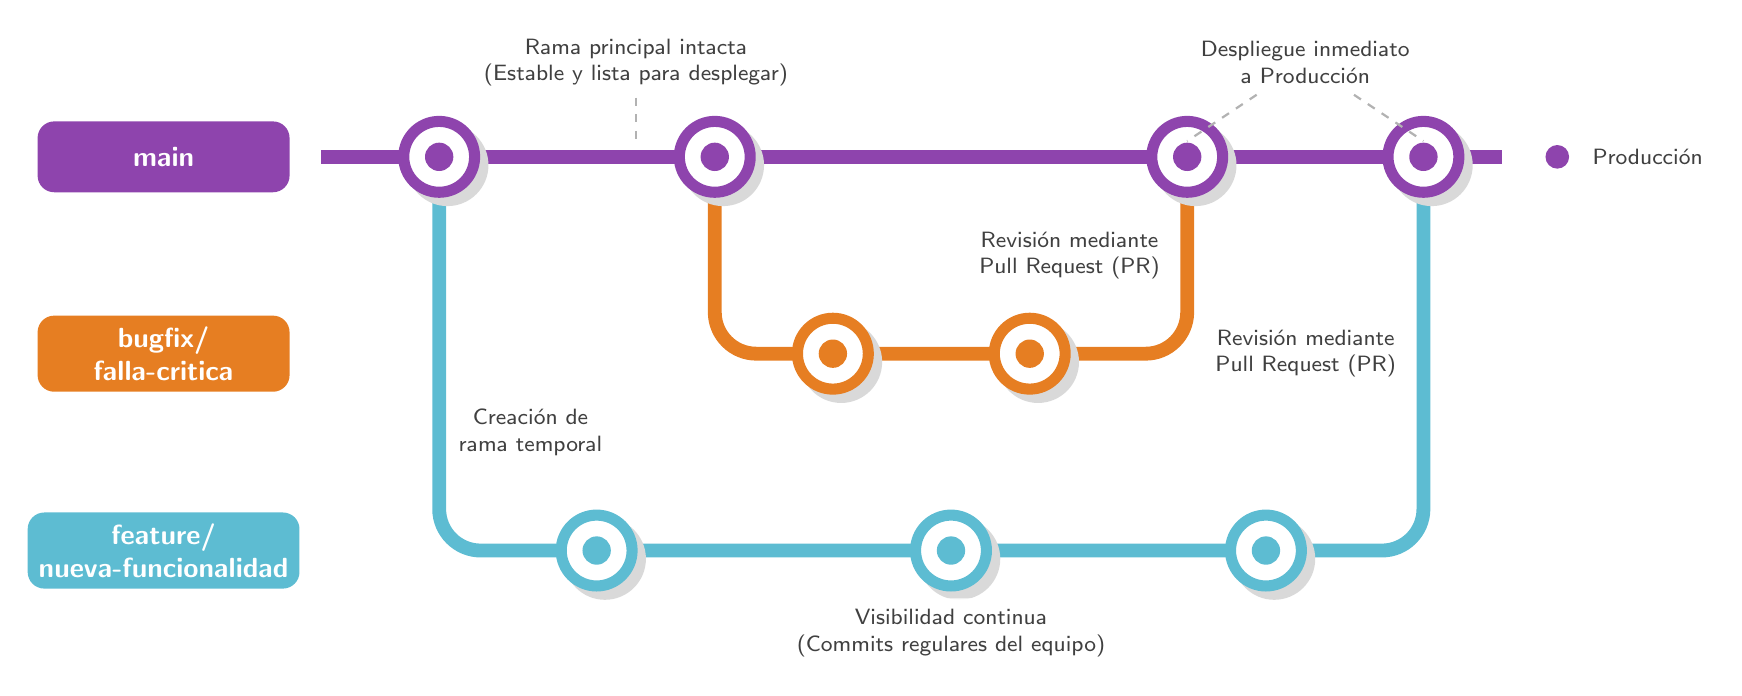
\begin{tikzpicture}[
    % ---------------------------------------------------------
    % ESTILOS BASE (DRY) - Sin saltos de línea vacíos
    % ---------------------------------------------------------
    commit/.style={
        circle, 
        draw=#1, 
        fill=white, 
        line width=4pt, 
        minimum size=0.9cm, 
        inner sep=0pt,
        general shadow={shadow xshift=3pt, shadow yshift=-3pt, fill=gray!30, draw=gray!30, line width=4pt},
        path picture={
            \fill[#1] (path picture bounding box.center) circle (0.18cm);
        }
    },
    path line/.style={
        draw=#1, 
        line width=5pt, 
        rounded corners=15pt
    },
    branch label/.style={
        rectangle, 
        rounded corners=6pt, 
        fill=#1, 
        text=white,
        font=\sffamily\bfseries, 
        align=center, 
        minimum width=3.2cm, 
        minimum height=0.9cm, 
        inner sep=4pt
    },
    annotation/.style={
        align=center,
        font=\sffamily\footnotesize\color{black!75},
        fill=white,
        fill opacity=0.9,
        text opacity=1,
        inner sep=4pt,
        rounded corners=4pt
    }
]

% ---------------------------------------------------------
% 1. COORDENADAS (Grid virtual)
% ---------------------------------------------------------
% main (Nivel Y = 0)
\coordinate (M1) at (1, 0);
\coordinate (M2) at (4.5, 0);
\coordinate (M3) at (10.5, 0); % Merge de bugfix
\coordinate (M4) at (13.5, 0); % Merge de feature

% bugfix (Nivel Y = -2.5)
\coordinate (B1) at (6, -2.5);
\coordinate (B2) at (8.5, -2.5);

% feature (Nivel Y = -5.0)
\coordinate (F1) at (3, -5);
\coordinate (F2) at (7.5, -5);
\coordinate (F3) at (11.5, -5);

% ---------------------------------------------------------
% 2. DIBUJO DE LÍNEAS
% ---------------------------------------------------------
% Línea main
\draw[path line=cPurple] (-0.5, 0) -- (14.5, 0);
\fill[cPurple] (15.2, 0) circle (0.15cm);

% Línea feature
\draw[path line=cCyan] (M1) |- (F1) -- (F3) -| (M4);

% Línea bugfix
\draw[path line=cOrange] (M2) |- (B1) -- (B2) -| (M3);

% ---------------------------------------------------------
% 3. NODOS (Commits superpuestos)
% ---------------------------------------------------------
% Commits de main
\node[commit=cPurple] at (M1) {};
\node[commit=cPurple] at (M2) {};
\node[commit=cPurple] at (M3) {};
\node[commit=cPurple] at (M4) {};

% Commits de bugfix
\node[commit=cOrange] at (B1) {};
\node[commit=cOrange] at (B2) {};

% Commits de feature
\node[commit=cCyan] at (F1) {};
\node[commit=cCyan] at (F2) {};
\node[commit=cCyan] at (F3) {};

% ---------------------------------------------------------
% 4. ETIQUETAS DE RAMAS 
% ---------------------------------------------------------
\node[branch label=cPurple] at (-2.5, 0) {main};
\node[branch label=cOrange] at (-2.5, -2.5) {bugfix/\\falla-critica};
\node[branch label=cCyan] at (-2.5, -5) {feature/\\nueva-funcionalidad};

% ---------------------------------------------------------
% 5. ANOTACIONES DE LOS PRINCIPIOS DE GITHUB FLOW
% ---------------------------------------------------------

% Principio 1: Rama principal intacta
\node[annotation] (lblMain) at (3.5, 1.2) {Rama principal intacta\\(Estable y lista para desplegar)};
\draw[dashed, gray!60, thick] (lblMain) -- (3.5, 0.2);

% Principio 2: Creación de ramas
\node[annotation, right=0.1cm] at (1, -3.5) {Creación de\\rama temporal};

% Principio 3: Visibilidad continua
\node[annotation, below=0.6cm] at (F2) {Visibilidad continua\\(Commits regulares del equipo)};

% Principio 4: Revisión mediante PR (Anotaciones en las líneas de integración)
\node[annotation, left=0.2cm] at (10.5, -1.25) {Revisión mediante\\Pull Request (PR)};
\node[annotation, left=0.2cm] at (13.5, -2.5) {Revisión mediante\\Pull Request (PR)};

% Principio 5: Despliegue inmediato
\node[annotation] (lblDeploy) at (12, 1.2) {Despliegue inmediato\\a Producción};
\draw[dashed, gray!60, thick] (lblDeploy) -- (10.5, 0.2);
\draw[dashed, gray!60, thick] (lblDeploy) -- (13.5, 0.2);

\node[annotation, right=0.3cm] at (15.2, 0) {Producción};

\end{tikzpicture}
\end{document}